% Copyright (c) 2008-2009 solvethis
% Copyright (c) 2010-2011 Casper Ti. Vector
% Public domain.

\chapter{GRT2.0系统及其射频通信库设计与实现}\label{chap:grt2.0}
	GRT2.0系统是本研究的前期工作,是本课题组合作完成的一款高性能可重构的软件无线电通信平台\cite{pkuraw},
	旨在帮助无线通信的软硬件研究与开发人员更好更快地在真实的通信系统中实现和验证无线通信系统物理层和MAC层的算法,
	GRT2.0系统是其最新的发布版本,应用有全双工\cite{mna16grt}、认知无线电\cite{fpga17grt}、低延迟通信等。
	本人负责其中射频通信库和工程自动化脚本,参与了LOW MAC模块的搭建。
	本节将对整体进行简单介绍,对本人完成的射频通信库的设计与实现进行具体展开。
	在\ref{sec:grt2.0_overview}小节介绍GRT2.0系统的整体框架,
	在\ref{sec:grt2.0_rfd}小节介绍射频通信库的设计,
	在\ref{sec:grt2.0_script}小节介绍工程自动化脚本,
	在\ref{sec:grt2.0_drawback}小节分析GRT2.0系统用于物理层WiFi安全研究时的不足,
	在\ref{sec:grt2.0_summary}小节对本节进行简单总结。

	\section{GRT2.0整体框架介绍}\label{sec:grt2.0_overview}
	在硬件组成上,GRT2.0系统包括四个部分,FPGA、上位主机、FPGA配置计算机、射频前端,
	如图\ref{fig:grt_overview}所示,
	其中上位主机与FPGA配置计算机可以是同一台计算机,各部分介绍如下:
		\begin{itemize}
			\item FPGA:作为无线电通信平台的核心数据处理硬件,包括射频通信库、物理层模块、LOW MAC模块、USB通信库四个部分,
			射频通信库负责射频前端的交互,
			物理层模块实现了802.11规定的物理层全部的数据处理过程,
			LOW MAC模块实现了802.11规定的MAC层的时序要求高的数据处理过程和控制流程,
			USB通信库负责与上位计算机的交互。
			\item 上位主机:运行GRT2.0的驱动,与上层网络协议栈连接,运行应用程序。
			\item FPGA配置计算机:FPGA的开发、烧写与调试。
			\item 射频前端:负责射频通信。
		\end{itemize}

		\begin{figure}
			\centering
			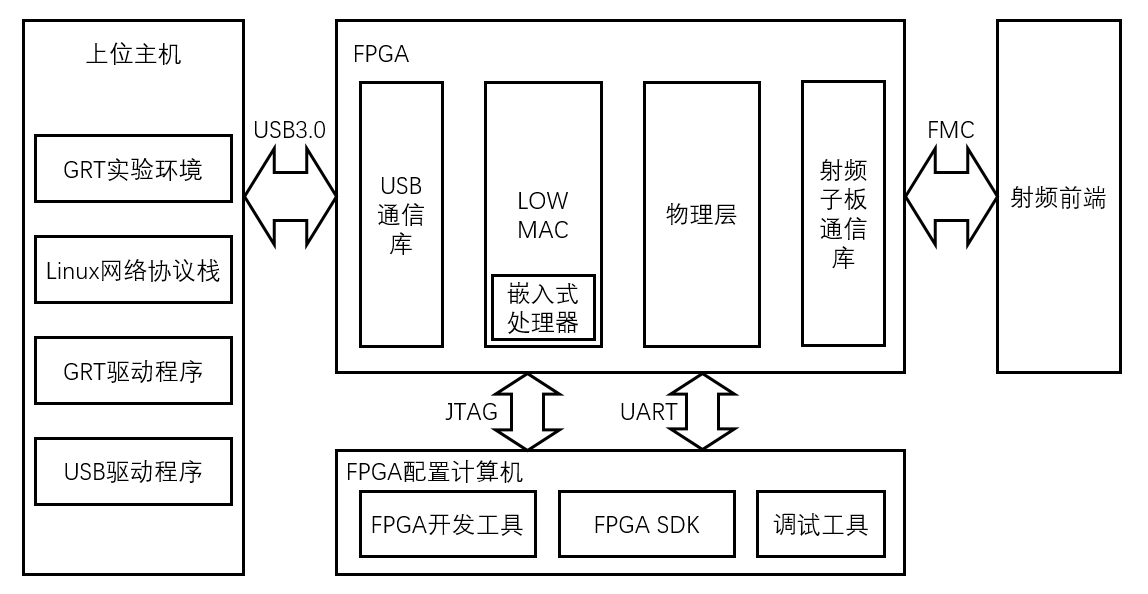
\includegraphics[width=1.0\textwidth]{img/GRT_overview.png}
			\caption{GRT2.0整体结构示意图}
			\label{fig:grt_overview}
		\end{figure}
	目前GRT2.0系统的FPGA部分使用的是Xilinx KC705开发板,后续版本也对Xilinx VC707进行了支持,
	上位主机使用的操作系统是Ubuntu14.04,
	FPGA配置计算机使用的开发工具是Vivado2015.2及其对应版本的SDK,
	射频前端使用的是Analog Device公司的EVAL-AD-FMCOMMS3-EBZ开发板\cite{fmcomms3}。

	值得一提的是,FPGA上的LOW MAC模块采用了软硬件协作的结构,
	将嵌入式处理器MicroBlaze\cite{microblaze}与硬件IP核\cite{xilinxip}结合,
	图\ref{fig:grt_lowmac}是LOW MAC模块软硬件协作的结构示意图,我参与了LOW MAC模块的搭建。
	硬件IP核是对完成特定功能的硬件逻辑的封装,
	嵌入式软件与硬件IP核结合的方式可以大大提高系统编程的灵活性。
	流程控制在嵌入式软件中实现,例如根据一帧的MAC地址进行分支处理,
	如果由硬件实现会非常繁琐,可读性和可扩展性差,
	数据通路和密集计算在硬件IP核中实现,例如发送端增加CRC校验位、接收端检测CRC是否匹配,
	硬件IP核可以每个时钟周期计算64bit的CRC,
	如果由软件实现会造成很高的延迟。
	在Vivado开发套件中,嵌入式处理器MicroBlaze与硬件IP核共同组织成block design\cite{xilinxblockdesign}的形式,具有图形化的开发界面。
	为了提高可编程性,本文在GRTSEC的设计中,也加入了软硬件协作的结构,第\ref{chap:grtsec_design}章会进行进一步介绍。

		\begin{figure}
			\centering
			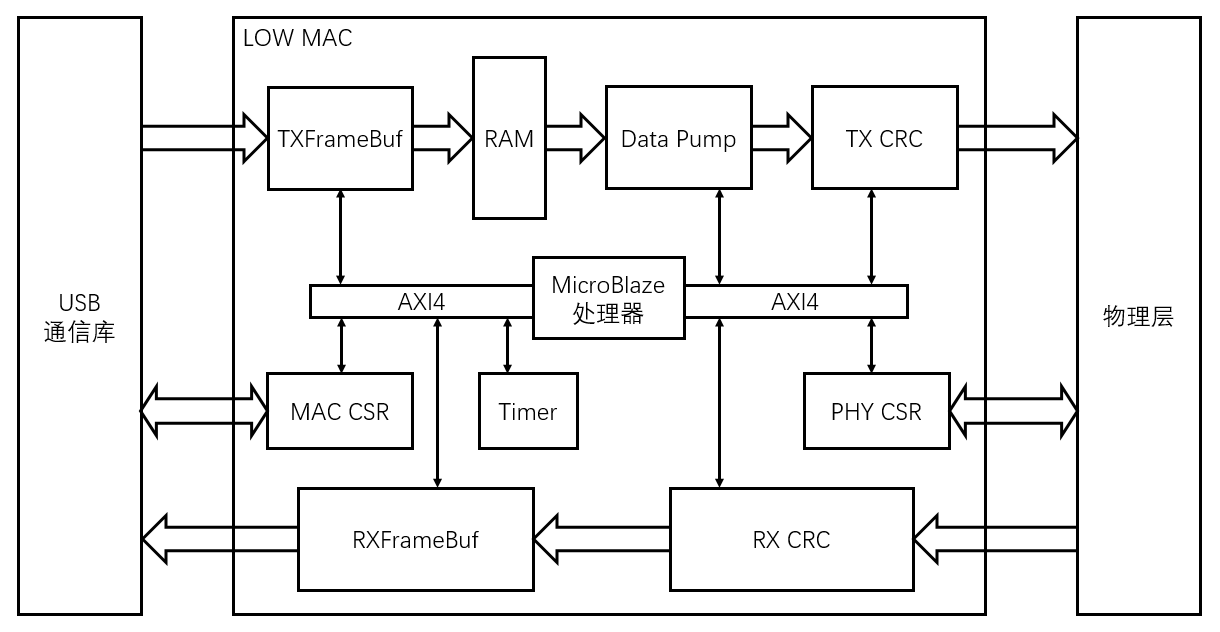
\includegraphics[width=1.0\textwidth]{img/GRT_lowmac.png}
			\caption{LOW MAC模块软硬件协同结构示意图}
			\label{fig:grt_lowmac}
		\end{figure}

	\section{射频通信库}\label{sec:grt2.0_rfd}
	射频前端是无线开放平台必备的组成部分,负责将数字基带信号转变为射频信号发送到空气中,
	以及接受空气中的射频信号转变为数字基带信号,射频前端的通信性能决定了无线平台的适用场景,
	对于WiFi无线验证平台,需要一个支持2.4GHz和5GHz中心频点、40MHz带宽的射频前端。
	作为一个提供给研究者的开放平台,除了考虑通信性能外,还要考虑价格,
	价格过高会让研究者望而却步。例如,OpenMili平台使用的射频前端\cite{mobicom16openmili}价格约11000美元,用于无线研究时价格过高。

	在GRT1.0系统中,我们选择使用USRP N210搭配XCVR2450子板\cite{usrpn210}作为射频前端,
	USRP N210价格是17000元,XCVR2450子板价格是4000元,属于可接受的范围。
	USRP的驱动是运行在Linux操作系统上的,称作UHD(USRP Hardware Driver),
	为了将FPGA开发板与射频前端相连,我们在FPGA上实现了USRP的硬件驱动,作为GRT1.0的射频通信库。
	这样的方式有以下几个缺点:
		\begin{itemize}
			\item XCVR2450子板最高支持25MHz带宽,无法达到802.11n协议要求的40MHz;
			\item USRP N210与FPGA开发板通过千兆以太网接口相连,
			以太网协议栈引入了不必要的延迟,经过GRT1.0射频通信库优化后的延迟也高达30ms以上,
			超过了802.11协议中要求的18ms的回复ACK的间隔,
			虽然可以与某些延迟要求宽松的商用设备实时通信,但系统的扩展性变得很差;
			\item 硬件实现USRP驱动的过程复杂,无法利用官方提供的软件驱动程序,也不方便驱动程序的升级换代;
			\item 不支持多天线MIMO(Multiple Input Multiple Output),MIMO技术是802.11n协议要求的技术。
		\end{itemize}

	以上缺点制约了无线平台的应用范围。

	在GRT2.0中,经过多方比较,我们选择使用性能更好、支持2x2 MIMO、具有通用接口的射频前端,
	Analog Device公司的EVAL-AD-FMCOMMS3-EBZ射频开发板\cite{fmcomms3},简称FMCOMMS3。
	FMCOMMS3的价格为6200元,射频芯片为Analog Device公司的AD9361,
	支持的中心频率范围是70MHz至6GHz,可以覆盖WiFi使用的2.4GHz和5GHz频段,
	带宽为200kHz至56MHz可调,支持802.11a协议要求的20MHz带宽、
	802.11b协议要求的18MHz带宽和802.11n协议要求的40MHz带宽,支持2x2 MIMO,
	通过高带宽的FMC接口(FPGA Mezzanine Card)\cite{wikifmc}与FPGA相连。
	虽然生产商提供了FPGA参考设计,但仍然无法直接与GRT系统集成,例如占用了过多的FPGA资源,没有提供上位主机配置射频参数的接口。
	射频通信库完成了GRT2.0系统与FMCOMMS3射频子板的对接。

	GRT2.0射频通信库的设计采用了嵌入式处理器与硬件IP核结合的方式。
	射频通信库软件部分所做的工作主要是对配置射频参数的接口进行封装,
	通过USB通信库与上位主机的驱动程序连接起来。
	由主机驱动程序配置的射频参数有中心频率和带宽,由射频通信库软件接口提供给主机驱动程序的是RSSI。

	射频通信库硬件部分对生产商提供的参考设计进行了较大的改造,体现在以下几点:
		\begin{itemize}
			\item 参考设计通过以太网与主机相连,通过HDMI与显示器相连,
			为降低FPGA资源使用率,射频通信库硬件部分去除对多种冗余接口的控制器,包括与主机相连的以太网接口控制器和以太网DMA控制器,
			与显示器相连的HDMI接口控制器,与板上LCD显示屏相连的LCD控制器,IIC接口控制器,只保留与FMC子板相连的FMC接口控制器;
			\item 参考设计将主机通过以太网发来的数据DMA到DDR3中,然后从DDR3中读取数据,
			经过AD9361 IP核转为时钟对齐的IQ两路数据,发送给FMCOMMS3子板,接收端与之方向相反,
			为降低数据传输延迟,射频通信库硬件部分去除收发数据读写DDR3的过程,直接转为FIFO接口与GRT系统的物理层模块相连;
			\item 参考设计中MicroBlaze配置级别高,性能好,
			为降低MicroBlaze占用的FPGA资源,射频通信库硬件部分简化了MicroBlaze的配置,
			提供支持射频通信库软件部分和LOW MAC软件部分的最小集合。
		\end{itemize}

	下面分别介绍射频通信库的数据通路的硬件接口和配置的嵌入式软件接口。
	在硬件设计中,射频通信库将AD9361 IP核输出的IQ两路数据转化为标准的FIFO接口,提供给物理层,并通过异步FIFO的方式完成时钟域转换。
	射频侧的时钟和复位信号由AD9361 IP核提供,这个时钟是随采样率变化的;物理层侧的时钟和复位信号由物理层提供。
	硬件接口以简单明了为目标,
	射频通信库与物理层之间的接口定义如下:
	\begin{lstlisting}[language={Verilog}]
module fmc_iface
(
input fmc_clk,
input fmc_rst,
input PHY_TX_clk,
input PHY_RX_clk,
input PHY_rst,
output PHY2RF_FIFO_prog_full,
input PHY2RF_FIFO_wr_en,
input [31:0] PHY2RF_FIFO_din,
input RF2PHY_FIFO_rd_en,
output [31:0] RF2PHY_FIFO_dout,
output RF2PHY_FIFO_empty,
output RF2PHY_FIFO_almost_empty
);
	\end{lstlisting}

	射频通信库在嵌入式软件端提供了配置射频参数接口。
	包括初始化射频子板,对射频子板的ADC、DAC、滤波器等初始化配置,设置中心频率、采样率、发送增益等射频参数。
	中心频率的单位是MHz,比如WiFi标准频段的信道1为2412MHz。
	采样率的单位为Sps(Samples per seconds),比如802.11a/g的采样率为20000000Sps,802.11n需要40000000Sps的模式。
	发送增益以衰减的形式表示,单位是mdb,即db的千分之一,设置为0时表示无衰减,1000时为衰减为十分之一。
	射频通信库提供的软件配置接口如下:
	\begin{lstlisting}[language={C}]
int fmc_main(void);
void set_rx_samp_freq(double* param, char param_no);
void set_tx_samp_freq(double* param, char param_no);
void set_rx_lo_freq(double* param, char param_no);
void set_tx_lo_freq(double* param, char param_no);
void set_tx1_attenuation(double* param, char param_no);
	\end{lstlisting}

	\section{工程自动化脚本}\label{sec:grt2.0_script}
	TCL脚本在FPGA的开发过程中有着广泛的运用\cite{xilinxtcl},从模块间引脚的连接、工程文件的组织,
	到调试信息的导出、自动执行工作流程,TCL脚本大大提高了FPGA开发的效率。
	为了将GRT2.0系统开源给研究者,我们提供了可以自动搭建工程项目的TCL脚本,
	实现了从源代码、资源文件到最终二进制文件的自动化过程。
	TCL脚本的使用是从GRT1.0到GRT2.0的一个重要改进。

	GRT2.0系统提供的工程自动化TCL脚本完成了以下过程:
		\begin{itemize}
			\item 对GRT2.0提供的完成特定功能的硬件逻辑封装成IP核;
			\item 生成block design中的各个模块和输入输出端口,完成模块间、端口间互相的连线;
			\item 生成和配置嵌入式处理器MicroBlaze及其附属的总线控制器,对总线地址进行分配;
			\item 对Xilinx提供的IP核进行配置,并添加到工程中,主要是各种不同类型的FIFO、时钟生成器、RAM、DDR3控制器等;
			\item 添加GRT2.0的资源文件,有约束文件、三角函数数据文件、OFDM导频数据文件等;
			\item 执行工作流程,设置流程策略,工作流程有综合(Synthesis)、布局(Place)、布线(Route)、生成二进制文件(Generate Bitstream)等。
		\end{itemize}

	通过执行工程自动化TCL脚本,用户可以利用手中的开发板和开源的GRT2.0代码,生成可以烧写FPGA的二进制文件,
	再结合我们提供的上位主机的驱动程序,用户便自行搭建GRT2.0系统完成。

	\section{用于安全研究时的不足}\label{sec:grt2.0_drawback}
	基于GRT2.0系统进行开发,可以满足设计目标中的与商用网卡实时通信,以及与上层网络协议栈连接,
	但在其他方面存在不足,尤其是无法获取物理层WiFi安全研究所需要的物理层信息。
	GRT2.0系统中物理层接收端的设计目标是消除接收信号的偏差,还原出发送信号,
	频偏纠正、相位纠正、信道均衡、Viterbi解码等过程都是为了完成这个目标,
	然而在物理层WiFi安全的研究中,接收信号的偏差有其背后的物理含义,常常被拿来做研究,
	但GRT2.0的系统框架不支持这些信息的提取。
	具体来说,用于安全研究时的不足包括以下几点。
		\begin{itemize}
			\item 物理层由单一的硬件逻辑实现,可编程性还不够高;
			\item 未提供方便获取CSI、RSSI的接口,CSI和RSSI是安全研究常用的指标;
			\item 在接收端数据处理过程中消除了信号偏差,而这些偏差在安全研究中常常被用到,例如频偏;
			\item 不支持软硬件数据处理模块替换的能力;
			\item 缺乏物理层编程的使用样例。
		\end{itemize}

	在第\ref{chap:grtsec_design}章将针对以上问题加以改进,
	介绍适用于物理层WiFi安全研究的验证平台GRTSEC的设计与实现。

	\section{本章小结}\label{sec:grt2.0_summary}
	本节对支持物理层WiFi安全研究的验证平台GRTSEC的前期工作GRT2.0系统进行了介绍,
	GRT2.0系统硬件上包括上位主机、FPGA、射频前端、配置计算机,
	由物理层模块、LOW MAC模块、射频通信库、USB通信库等模块组成。
	GRT2.0系统可以满足本文设计目标中的与商用网卡实时通信,以及与上层网络协议栈连接,
	但在获取物理层信息、物理层编程性、软硬件模块替换等方面存在不足。
	另外,本节展开介绍了本人在GRT2.0系统中完成的工作,主要负责完成的射频通信库、工程自动化脚本,
	参与完成的LOW MAC软硬件协作设计。
